
\documentclass[%
  pdf,
  colorBG,
  slideColor,
% draft,
% nologo,
  frames,
  ogf
]{prosper}

\usepackage{fancyvrb}
\usepackage{xspace}

\newcommand{\T}[1]{\texttt{#1}}
\newcommand{\I}[1]{\textit{#1}}
\newcommand{\B}[1]{\textbf{#1}}
\newcommand{\U}[1]{\underline{#1}}
\newcommand{\F}[1]{\B{FIXME: #1}}

\newcommand{\LRA}{$\longrightarrow$~~}
\newcommand{\LLA}{$\longleftarrow$~~}
\newcommand{\RA}{$\rightarrow$~~}
\newcommand{\LA}{$\leftarrow$~~}

\newcommand{\up}{\vspace*{-1em}}
\newcommand{\dn}{\vspace*{+1em}}

\newcommand{\lf}{look\,\&\,feel\xspace}

\DefineVerbatimEnvironment{mycode}{Verbatim}
{
  label=Code Example,
  fontsize=\tiny,
  frame=single,
% framerule=1pt,
% framesep=1em,
% numbers=left,
  gobble=2
}


\title{\flushleft SAGA Tutorial - NeSC 2009}
\author{\LARGE \white Introduction to the SAGA API}
\slideCaption{-- NeSC, Edinburgh, September 3rd 2009 --}

\setlength{\baselineskip}{-1em}

%%%%%%%%%%%%%%%%%%%%%%%%%%%%%%%%%%%%%%%%%%%%%%%%%%%%%%%%%%%%

\begin{document}

 \slidetitlepage
 %%%%%%%%%%%%%%%%%%%%%%%%%%%%%%%%%%%%%%%%%%%%%%%%%%%%%%%%%%%

 \begin{slide}{Agenda}

  \dn

  \begin{itemize}
   \item Background Recap
   \item SAGA API structure and scope
   \item walkthrough
   \item some implementation details
   \item SAGA extensions
  \end{itemize}

 \end{slide}

 %%%%%%%%%%%%%%%%%%%%%%%%%%%%%%%%%%%%%%%%%%%%%%%%%%%%%%%%%%%%

 \begin{slide}{Grid APIs and Frameworks}

 \dn

  \begin{itemize}
   \item Middleware often targets legacy applications (Unicore, Globus, Condor, ...)
   \item some are distribution aware (MPICH-G, Ninf-G, \dots)
   \item few \B{A}PIs exist for Grid aware applications
    \begin{itemize}
     \item GridFTP
     \item GRAM
     \item gLite
     \item CoG
     \item GAT
     \item Cloud APIs
    \end{itemize}
  \end{itemize}

 \end{slide}

 %%%%%%%%%%%%%%%%%%%%%%%%%%%%%%%%%%%%%%%%%%%%%%%%%%%%%%%%%%%

 \begin{slide}{Grid APIs and Frameworks}
 \dn
  \begin{itemize}
   \item diversity of Grid Middleware implies diversity of APIs
   \item some APIs try to generalize Grid programming concepts
   \item difficult to keep up with MW development, and to stay \B{simple}
  \end{itemize}
 \end{slide}

 %%%%%%%%%%%%%%%%%%%%%%%%%%%%%%%%%%%%%%%%%%%%%%%%%%%%%%%%%%%

 \begin{slide}{OGF}
 \dn
  \begin{itemize}
   \item Open Grid Forum (GF, EGF, GGF) tries to standardize Grid MW
   \item e.g. single job description language (JSDL)
   \item focuses on interfaces, but also protocol and architecture
  \end{itemize}
 \end{slide}

 %%%%%%%%%%%%%%%%%%%%%%%%%%%%%%%%%%%%%%%%%%%%%%%%%%%%%%%%%%%

 \begin{slide}{APIs within OGF}

 \dn 

  \begin{itemize}
   \item OGF focuses on services
   \item some effort on higher level APIs
   \begin{itemize}
    \item Distributed Resource Management Application API (DRMAA)
    \item Remote Procedure Calls (GridRPC)
    \item Checkpoint and Recovery (GridCPR)
    \item Job Submission and Description Language (JSDL)
   \end{itemize}
   \item numerous service interfaces, often WS-based (WSRF)
  \end{itemize}

 \end{slide}

 %%%%%%%%%%%%%%%%%%%%%%%%%%%%%%%%%%%%%%%%%%%%%%%%%%%%%%%%%%%

 \begin{slide}{OGF: DRMAA}

 \dn 

  \begin{itemize}
   \item implementable on all major resource management services
   \item simple means to define jobs, and to submit them
   \item basic job management features (status, kill)
   \item job templates for bulk job management
  \end{itemize}

 \end{slide}

 %%%%%%%%%%%%%%%%%%%%%%%%%%%%%%%%%%%%%%%%%%%%%%%%%%%%%%%%%%%

 \begin{slide}{DRMAA Example}

  \begin{mycode}[label=DRMAA Job Submit]
  drmaa_job_template_t * job_template;

  if ( ! ( job_template = create_job_template (exe, 5, 0) ) ) 
  {
    fprintf (stderr, "create_job_template failed\n");
    return 1;
  }

  while ( ( drmaa_errno = drmaa_run_job (job_id, 
                                         sizeof (jobid)-1, 
                                         job_template, 
                                         diagnosis, 
                                         sizeof (diagnosis)-1)
          ) == DRMAA_ERRNO_DRM_COMMUNICATION_FAILURE )
  {
    fprintf(stderr, "drmaa_run_job failed: %s\n", diagnosis);
    sleep (1);
  }
  \end{mycode}

 \end{slide}

 %%%%%%%%%%%%%%%%%%%%%%%%%%%%%%%%%%%%%%%%%%%%%%%%%%%%%%%%%%%

 \begin{slide}{OGF: GridRPC}

 \dn 

  \begin{itemize}
   \item 'standardizes' the three existing RPC implementations for Grids
   \item example of \I{'gridified API'}
   \item simple: get function handle, call function
   \item explicit support for async rpc calls
  \end{itemize}

 \end{slide}

 %%%%%%%%%%%%%%%%%%%%%%%%%%%%%%%%%%%%%%%%%%%%%%%%%%%%%%%%%%%

 \begin{slide}{OGF: GridRPC}

  \begin{mycode}[label=GridRPC: Matrix Multiplication]
  double A[N*N], B[N*N], C[N*N];
 
  initMatA (N, A);   
  initMatB (N, B);
 
  grpc_initialize (argv[1]);

  grpc_function_handle_t handle;
  grpc_function_handle_default (&handle, "mat_mult");
 
  if ( grpc_call (&handle, N, A, B, C) != GRPC_NO_ERROR) 
  {
    exit (1);
  }
 
  grpc_function_handle_destruct (&handle);
  grpc_finalize ();
  \end{mycode}

 \end{slide}

 %%%%%%%%%%%%%%%%%%%%%%%%%%%%%%%%%%%%%%%%%%%%%%%%%%%%%%%%%%%

 \begin{slide}{OGF: GridCPR}

 \dn 

  \begin{itemize}
   \item Grids seem to favour application level checkpointing
   \item GridCPR allows to manage checkpoints 
   \item defines an architecture, service interfaces,\\
         and, aehem, no API
  \end{itemize}

 \end{slide}

 %%%%%%%%%%%%%%%%%%%%%%%%%%%%%%%%%%%%%%%%%%%%%%%%%%%%%%%%%%%

 \begin{slide}{OGF: JSDL}

 \dn 

  \begin{itemize}
   \item extensible XML based language for describing job requirements
   \item does not cover resource description (on purpose)
   \item does not cover workflows, or job dependencies etc (on purpose)
   \item JSDL is extensible (ParameterSweep, SPMD)
  \end{itemize}

 \end{slide}

 %%%%%%%%%%%%%%%%%%%%%%%%%%%%%%%%%%%%%%%%%%%%%%%%%%%%%%%%%%%

 \begin{slide}{OGF: JSDL}

  \begin{mycode}[label=JSDL: Simple Job]
   <jsdl:JobDefinition>
     <JobDescription>
        <Application>
           <jsdl-posix:POSIXApplication>
              <Executable>/bin/date</Executable>
           </jsdl-posix:POSIXApplication>
        </Application>
        <Resources ...>
           <OperatingSystem>
              <OperatingSystemType>
                 <OperatingSystemName>LINUX</OperatingSystemName>
              </OperatingSystemType>
           </OperatingSystem>
        </Resources>
     </JobDescription>
  <jsdl:JobDefinition>
  \end{mycode}

 \end{slide}

 %%%%%%%%%%%%%%%%%%%%%%%%%%%%%%%%%%%%%%%%%%%%%%%%%%%%%%%%%%%

 \begin{slide}{OGF: JSDL}

  \dn 

  \begin{itemize}
   \item XML: embeddable into WSRF (WS-Agreement etc.)
   \item XML, but relatively flat
   \item maps well to existing JDLs, but is 'more complete'
   \item extensible (resource description, job dependencies, workflow)
   \item top down approach!
  \end{itemize}

 \end{slide}

 %%%%%%%%%%%%%%%%%%%%%%%%%%%%%%%%%%%%%%%%%%%%%%%%%%%%%%%%%%%

 \begin{slide}{OGF: Summary}

  \dn 

  \begin{itemize}
   \item some APIs exist in OGF, and are successfull
   \item OGF APIs do not cover the complete OGF scope
   \item the various API standards are disjunct
   \item WSDL as service interface specification cannot replace an application
   level API (wrong level of abstraction)
   \item \B{SAGA tries to address these issues}
  \end{itemize}

 \end{slide}

 %%%%%%%%%%%%%%%%%%%%%%%%%%%%%%%%%%%%%%%%%%%%%%%%%%%%%%%%%%%

 \begin{slide}{OGF: top-down vs. bottom-up}

  \dn 

  \begin{itemize}
   \item bottom-up often agrees on (semantic) LCD + backend specific extensions
   \item top-down usually focuses on semantics of application
   requirements\\[2em]

   \item bottom-up tends to be more powerful
   \item top-down tends to be simplier and more concise\\[2em]

   \item \I{we very much prefer top-down!}
  \end{itemize}

 \end{slide}

 %%%%%%%%%%%%%%%%%%%%%%%%%%%%%%%%%%%%%%%%%%%%%%%%%%%%%%%%%%%
 
 \begin{slide}{SAGA}
 
  \dn\dn\dn\dn\dn
 
  \begin{center}
   \Huge \B{SAGA}\\[10mm]
   \Large Simple API for Grid Applications
  \end{center}
 
 \end{slide}
 
 %%%%%%%%%%%%%%%%%%%%%%%%%%%%%%%%%%%%%%%%%%%%%%%%%%%%%%%%%%%

 \begin{slide}{SAGA Design Principles}

  \begin{itemize}
   \item \B{SAGA}: \B{S}imple \B{A}PI for \B{G}rid \B{A}pplications
   \item OGF approach to a uniform API layer (facade)
   \item \B{governing principle:} \B{80:20 rule}\\
   simplicity versus control!
   \item \B{top-down approach:} use case driven!\\
         \RA defines \B{application level} abstractions
   \item \B{extensible:} stable \lf + API packages
   \item \B{influenced by:} DRMAA, GridRPC, OREP, JSDL,
         POSIX, GAT, CoG, LSF, Globus, \dots
   \item API Specification is \B{Language Independent} (IDL)\\
   Renderings exist in C++, Python, Java\\
   Examples here are in C++
  \end{itemize}

 \end{slide}

 %%%%%%%%%%%%%%%%%%%%%%%%%%%%%%%%%%%%%%%%%%%%%%%%%%%%%%%%%%%

 \begin{slide}{SAGA Intro: Example 1}
  
  \begin{mycode}[label=SAGA: File Management]

  saga::filesystem::directory dir ("any://remote.host.net//data/");

  if ( dir.exists ("a") && ! dir.is_dir ("a") )
  {
    dir.copy ("a", "b", Overwrite);
  }

  list <saga::url> names = dir.find ("*-{123}.txt");

  saga::filesystem::directory tmp  = dir.open_dir ("tmp/", Create);
  saga::filesystem::file      file = dir.open     ("tmp/data.txt");

  \end{mycode}
   
 \end{slide}


 %%%%%%%%%%%%%%%%%%%%%%%%%%%%%%%%%%%%%%%%%%%%%%%%%%%%%%%%%%%

 \begin{slide}{SAGA Intro: Example 1}

  \dn\dn
  
  \begin{itemize}
   \item API is clearly POSIX (libc + shell) inspired
   \item where is my security??
   \item what is '\T{any://}' ???
  \end{itemize}

 \end{slide}


 %%%%%%%%%%%%%%%%%%%%%%%%%%%%%%%%%%%%%%%%%%%%%%%%%%%%%%%%%%%

 \begin{slide}{SAGA Intro: Example 2}

  \begin{mycode}[label=SAGA: Job Submission]

  saga::job::description jd; // details left out 
  saga::job::service     js ("any://remote.host.net/");
  saga::job::job         j = js.create_job (jd);

  j.run ();

  cout << "Job State: " << j.get_state () << endl;

  j.wait ();

  cout << "Retval " << j.get_attribute ("ExitCode") << endl;

  \end{mycode}
   
 \end{slide}


 %%%%%%%%%%%%%%%%%%%%%%%%%%%%%%%%%%%%%%%%%%%%%%%%%%%%%%%%%%%

 \begin{slide}{SAGA Intro: Example 2'}

  \begin{mycode}[label=SAGA: Job Submission]


  saga::job::service     js ("any://remote.host.net");
  saga::job::job         j = js.run_job ("touch /tmp/touch.me");



  cout << "Job State: " << j.get_state () << endl;

  j.wait ();

  cout << "Retval " << j.get_attribute ("ExitCode") << endl;

  \end{mycode}
   
 \end{slide}


 %%%%%%%%%%%%%%%%%%%%%%%%%%%%%%%%%%%%%%%%%%%%%%%%%%%%%%%%%%%

 \begin{slide}{SAGA Intro: Example 2}

  \dn\dn
  
  \begin{itemize}
   \item stateful objects!
   \item yet another job description langauge? \T{:-(}
   \item many hidden/default parameters (to keep call signatures 
   small)
   \item '\T{any://}' again!
   \item TIMTOWTDI (there is more than one way to do it)
  \end{itemize}

 \end{slide}


 %%%%%%%%%%%%%%%%%%%%%%%%%%%%%%%%%%%%%%%%%%%%%%%%%%%%%%%%%%%

 \begin{slide}{SAGA Intro: 10.000 feet}

  \begin{itemize}
   
   \item \B{object oriented:} inheritance, interfaces\\
   very moderate use of templates though!

   \item functional and non-functional elements strictly separated

    \begin{itemize}

     \item \I{non-functional API:} \lf - orthogonal to functional API\\
     often not mappable to remote operations

     \item \I{functional API:} API 'Packages' - extensible\\
     typically mappable to remote operations

    \end{itemize}

   \item few inter-package dependencies - allows for partial implementations

  \end{itemize}

 \end{slide}


 %%%%%%%%%%%%%%%%%%%%%%%%%%%%%%%%%%%%%%%%%%%%%%%%%%%%%%%%%%%

 \begin{slide}{SAGA: Class hierarchy}
  \begin{center}
   \includegraphics[width=\textwidth]{Pics/classes-10.eps}
  \end{center}
  {\footnotesize\B{SAGA API Structure:} \lf (top) + API packages (bottom)}
 \end{slide}
 
 %%%%%%%%%%%%%%%%%%%%%%%%%%%%%%%%%%%%%%%%%%%%%%%%%%%%%%%%%%%
 
 \begin{slide}{Implementation}
   \includegraphics[width=\textwidth]{Pics/saga_architecture.eps}
 \end{slide}


 %%%%%%%%%%%%%%%%%%%%%%%%%%%%%%%%%%%%%%%%%%%%%%%%%%%%%%%%%%%


 %%%%%%%%%%%%%%%%%%%%%%%%%%%%%%%%%%%%%%%%%%%%%%%%%%%%%%%%%%%

 \overlays{11}{
  \begin{slide}{SAGA: Class hierarchy}
   \begin{center}
    \onlySlide*{1}{\includegraphics[width=\textwidth]{Pics/classes-0.eps}}
    \onlySlide*{2}{\includegraphics[width=\textwidth]{Pics/classes-1.eps}}
    \onlySlide*{3}{\includegraphics[width=\textwidth]{Pics/classes-2.eps}}
    \onlySlide*{4}{\includegraphics[width=\textwidth]{Pics/classes-3.eps}}
    \onlySlide*{5}{\includegraphics[width=\textwidth]{Pics/classes-4.eps}}
    \onlySlide*{6}{\includegraphics[width=\textwidth]{Pics/classes-5.eps}}
    \onlySlide*{7}{\includegraphics[width=\textwidth]{Pics/classes-6.eps}}
    \onlySlide*{8}{\includegraphics[width=\textwidth]{Pics/classes-7.eps}}
    \onlySlide*{9}{\includegraphics[width=\textwidth]{Pics/classes-8.eps}}
    \onlySlide*{10}{\includegraphics[width=\textwidth]{Pics/classes-9.eps}}
    \onlySlide*{11}{\includegraphics[width=\textwidth]{Pics/classes-10.eps}}
   \end{center}
   \onlySlide*{2}{\B{SAGA Look \& Feel:}\\
                  \T{saga::object} allows for object uuids, \T{clone()} etc.}
   \onlySlide*{3}{\B{SAGA Look \& Feel:}\\
                  errors are based on exceptions or error codes.}
   \onlySlide*{4}{\B{SAGA Look \& Feel:}\\
                  session and credential management is hidden.}
   \onlySlide*{5}{\B{SAGA Look \& Feel:}\\
                  Attribute interface for meta data.}
   \onlySlide*{6}{\B{SAGA Look \& Feel:}\\
                  Monitoring includes asynchronous notifications.}
   \onlySlide*{7}{\B{SAGA Look \& Feel:}\\
                  the task model adds asynchronous operations.}
   \onlySlide*{8}{\B{SAGA API Package 'job':}\\
                  create and manage remote processes.}
   \onlySlide*{9}{\B{SAGA API Package 'name\_spaces':}\\
                  manage files, replicas, etc.}
   \onlySlide*{10}{\B{SAGA API Package 'stream':}\\
                  SAGA rendering of BSD streams.}
   \onlySlide*{11}{~\\\B{SAGA API Package 'rpc':}\\
                  remote procedure calls.}
  \end{slide}
 } % end overlays

 %%%%%%%%%%%%%%%%%%%%%%%%%%%%%%%%%%%%%%%%%%%%%%%%%%%%%%%%%%%

 \begin{slide}{SAGA}
   
   \dn\dn\dn\dn\dn 
   
   \begin{center}
   
     \B{\large Functional API Packages}

   \end{center}

 \end{slide}

 %%%%%%%%%%%%%%%%%%%%%%%%%%%%%%%%%%%%%%%%%%%%%%%%%%%%%%%%%%%

 \begin{slide}{SAGA: Jobs}
   \includegraphics[width=\textwidth]{Pics/classes-7.eps}
 \end{slide}

 %%%%%%%%%%%%%%%%%%%%%%%%%%%%%%%%%%%%%%%%%%%%%%%%%%%%%%%%%%%

 \begin{slide}{SAGA: Jobs - Overview}

 \dn 

  \begin{itemize}
   \item \T{job\_service} uses \T{job\_description} to create \T{job} instances
   \item \T{job\_description} attributes are based on JSDL 
   \item state model is based on / synced with BES
   \item \T{job\_self} represents the SAGA application
   \item job submission and management, but no resource discovery, job
   dependencies, or workflows
  \end{itemize}

 \end{slide}

 %%%%%%%%%%%%%%%%%%%%%%%%%%%%%%%%%%%%%%%%%%%%%%%%%%%%%%%%%%%

 \begin{slide}{SAGA: Job States}
  \begin{center}
   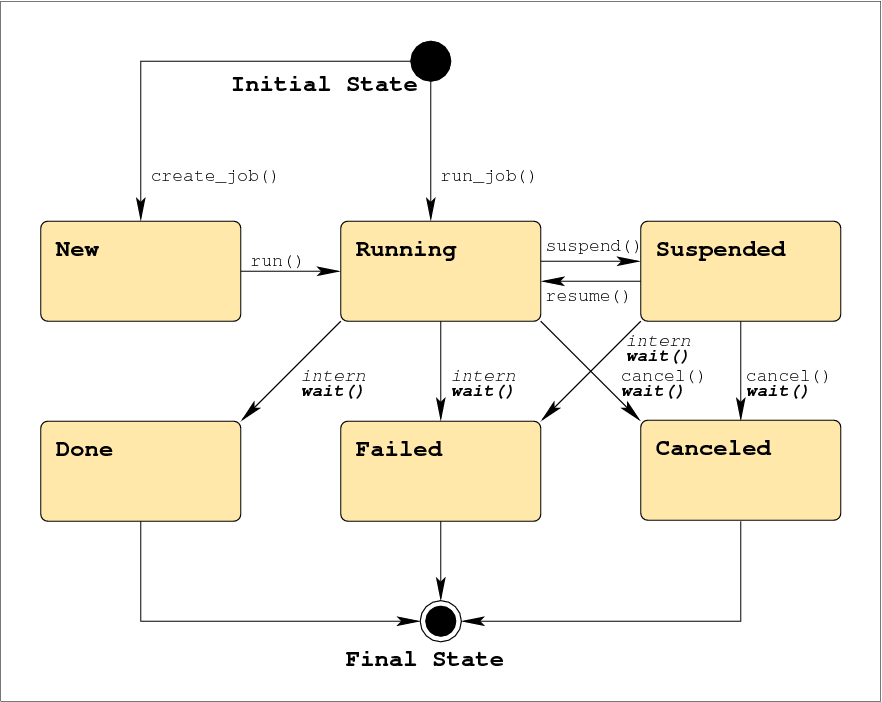
\includegraphics[height=\textheight]{Pics/job_states.eps}
  \end{center}
 \end{slide}

 %%%%%%%%%%%%%%%%%%%%%%%%%%%%%%%%%%%%%%%%%%%%%%%%%%%%%%%%%%%

 \begin{slide}{SAGA Examples: Jobs}

  \begin{mycode}[label=job submission]

  
  saga::job::service     js ("gram://headnode.gram.net");
  saga::job::job         j = js.run_job ("/bin/sleep 10", 
                                        "clusternode-2.gram.net");


  cout << "Job State: " << j.get_state () << endl;

  j.wait ();

  cout << "Retval " << j.get_attribute ("ExitCode") << endl;

  \end{mycode}
   
 \end{slide}

 %%%%%%%%%%%%%%%%%%%%%%%%%%%%%%%%%%%%%%%%%%%%%%%%%%%%%%%%%%%

 \begin{slide}{SAGA Examples: Jobs}

  \begin{mycode}[label=job submission]

  saga::job::description jd;
  saga::job::service     js ("gram://remote.host.net");
  saga::job              j = js.create_job (jd);

  j.run ();

  cout << "Job State: " << j.get_state () << endl;

  j.wait ();

  cout << "Retval " << j.get_attribute ("ExitCode") << endl;

  \end{mycode}
   
 \end{slide}

 %%%%%%%%%%%%%%%%%%%%%%%%%%%%%%%%%%%%%%%%%%%%%%%%%%%%%%%%%%%

 \begin{slide}{SAGA Examples: Jobs}

  \begin{mycode}[label=jobs (cont.)]

  j.run     ();
  j.wait    ();
  j.cancel  ();

  j.suspend ();
  j.resume  ();

  j.signal     (SIGUSR1);
  j.checkpoint ();
  j.migrate    (jd);

  \end{mycode}
   
 \end{slide}

 %%%%%%%%%%%%%%%%%%%%%%%%%%%%%%%%%%%%%%%%%%%%%%%%%%%%%%%%%%%

 \begin{slide}{SAGA Examples: Job Descr.}

  \begin{mycode}[label=job description - JSDL based]

  saga::job::description jd;

  jd.set_attribute ("Executable",       "/bin/tail");
  jd.set_attribute ("WorkingDirectory", "data/");
  jd.set_attribute ("Cleanup",          "False");

  // pseudo code *blush*
  jd.set_vector_attribute ("Arguments",    ["-f", "my_log"]);
  jd.set_vector_attribute ("Environment",  ["TMPDIR=/tmp/"]);
  jd.set_vector_attribute ("FileTransfer", ["my_log >> all_logs"]);

  \end{mycode}
   
 \end{slide}

 %%%%%%%%%%%%%%%%%%%%%%%%%%%%%%%%%%%%%%%%%%%%%%%%%%%%%%%%%%%

 \begin{slide}{SAGA Job Description}

  SAGA JD attributes:

  \begin{tabbing}
  XXXXXXXXXXXXXXX    \= XXXXXXXXXXXXX     \= \kill       

  Executable          \> Arguments           \> Environment         \\
  CandidateHosts      \> SPMDVariation       \> TotalCPUCount       \\
  NumberOfProcesses   \> ProcessesPerHost    \> ThreadsPerProcess   \\
  WorkingDirectory    \> \I{Interactive}     \> Cleanup             \\
  Input               \> Output              \> Error               \\
  \I{JobStartTime}    \> WallTimeLimit       \> TotalCPUTime        \\
  TotalPhysicalMemory \> CPUArchitecture     \> OperatingSystemType \\
  \I{Queue}           \> JobProject          \> \I{JobContact}      \\
  FileTransfer                                                      \\

  \end{tabbing}

 \end{slide}


 %%%%%%%%%%%%%%%%%%%%%%%%%%%%%%%%%%%%%%%%%%%%%%%%%%%%%%%%%%%

 \begin{slide}{SAGA Job Description}

  \dn

  \begin{itemize}

   \item leaning heavily on \B{JSDL}, but flat
   \item borrowing from DRMAA
   \item mixes hardware, software and scheduling attributes!
   \item cannot be extended
   \item no support for 'native' job descriptions (RSL, JDL, ...)
   \item only '\T{Executable}' is required
   \item backend MAY ignore unsupported keys!\footnote{\tiny{\T{cd /tmp/data \&\& rm
   -rf *}}}

  \end{itemize}

 \end{slide}

 %%%%%%%%%%%%%%%%%%%%%%%%%%%%%%%%%%%%%%%%%%%%%%%%%%%%%%%%%%%
 
 \begin{slide}{SAGA Example: job service}

  \begin{mycode}[label=job service]

  saga::job::service js ("gram://remote.host.net/");
 
  vector<string> ids = js.list (); // list known jobs
 
  while ( ids.size () )
  {
    string id = ids.pop_back ();

    saga::job j = js.get_job (id);  // reconnect to job
    
    cout << id << " : " << j.get_state () << endl;
  }
  \end{mycode}
   
 \end{slide}
 
 
 %%%%%%%%%%%%%%%%%%%%%%%%%%%%%%%%%%%%%%%%%%%%%%%%%%%%%%%%%%%

 \begin{slide}{SAGA Job Service}

  \dn

  \begin{itemize}

   \item represents a specific job submission endpoint
   \item job states are maintained on that endpoint (usually)
   \item full reconnect may not be possible (I/O streaming)
   \item lifetime of state up to backend
   \item reconnected jobs may have different job description (lossy translation)

  \end{itemize}

 \end{slide}

 %%%%%%%%%%%%%%%%%%%%%%%%%%%%%%%%%%%%%%%%%%%%%%%%%%%%%%%%%%%
 
 \begin{slide}{SAGA Examples: Job 'Self'}
 
  \begin{mycode}[label=jobs (cont.)]
 
  saga::job::self self = js.get_self ();
 
  self.signal     (SIGUSR1);
  self.checkpoint ();
  self.migrate    (jd);
  
  self.wait   ();   // blocks forever :-P
  self.cancel ();
 
  \end{mycode}
   
 \end{slide}


 %%%%%%%%%%%%%%%%%%%%%%%%%%%%%%%%%%%%%%%%%%%%%%%%%%%%%%%%%%%

 \begin{slide}{SAGA Job Self}

  \dn

  \begin{itemize}

   \item represents the \B{calling application instance}
   \item \T{self.signal (SIGUSR1);}\\
         ~~~ is different from\\ 
         \T{::kill (::getpid (), SIGUSR1);}\\
         ~~~ as it goes over the job manager (accounting,\\
         ~~~ logging, cleanup...)
   \item '\T{job::self}' is the only SAGA object to which metrics can be added
   (details later...)

  \end{itemize}

 \end{slide}

 %%%%%%%%%%%%%%%%%%%%%%%%%%%%%%%%%%%%%%%%%%%%%%%%%%%%%%%%%%%

 \begin{slide}{SAGA: Name Spaces etc.}
   \includegraphics[width=\textwidth]{Pics/classes-8.eps}
 \end{slide}

 %%%%%%%%%%%%%%%%%%%%%%%%%%%%%%%%%%%%%%%%%%%%%%%%%%%%%%%%%%%

 \begin{slide}{SAGA: Name Spaces}

 \dn 

  \begin{itemize}
   \item interfaces for managing entities in name spaces
   \item files, replicas, information, resources, steering parameter,
         checkpoints, \dots
   \item manages hierarchy (mkdir, cd, ls, \dots)
   \item manages NS entries as opaque (copy, move, delete, ...)
  \end{itemize}

 \end{slide}

 %%%%%%%%%%%%%%%%%%%%%%%%%%%%%%%%%%%%%%%%%%%%%%%%%%%%%%%%%%%

 \begin{slide}{SAGA: Files}

 \dn 

  \begin{itemize}
   \item implements name space interface, and adds access to content of NS
         entries (files)
   \item Posix oriented: read, write seek
   \item Grid optimizations: scattered I/O, pattern based I/O, extended I/O
  \end{itemize}

 \end{slide}

 %%%%%%%%%%%%%%%%%%%%%%%%%%%%%%%%%%%%%%%%%%%%%%%%%%%%%%%%%%%

 \begin{slide}{SAGA: Replicas}

 \dn 

  \begin{itemize}
   \item implements name space interface, and adds access to properties of NS
         entries (logical files / replicas)
   \item O/REP oriented: list, add, remove replicas; manage meta data
   \item Grid optimizations are hidden (replica placement strategies,
         consistency and version management, \dots)
  \end{itemize}

 \end{slide}

 %%%%%%%%%%%%%%%%%%%%%%%%%%%%%%%%%%%%%%%%%%%%%%%%%%%%%%%%%%%

 \begin{slide}{SAGA: Adverts}

 \dn 

  \begin{itemize}
   \item implements name space interface, and adds access to 
         arbitrary key/value pairs on each entry.  
   \item entries also allow to store a \B{serialized} SAGA Object!
   \item utterly useful for application bootstrapping,
   communication between different application modules,
   application persistency, etc etc.
   \item \B{not part of the SAGA Specification}, but is getting
   standardized as an extension
  \end{itemize}

 \end{slide}

 %%%%%%%%%%%%%%%%%%%%%%%%%%%%%%%%%%%%%%%%%%%%%%%%%%%%%%%%%%%


 \begin{slide}{SAGA Examples: NameSpaces}

  \begin{mycode}[label=name space management]

  saga::name_space::directory d ("ssh://remote.host.net//data/");

  if ( d.is_entry ("a") && ! d.is_dir ("a") )
  {
    d.copy ("a", "../b");
    d.link ("../b", "a", Overwrite);
  }

  list <saga::url> names = d.find ("*-{123}.text.");

  saga::name_space::directory tmp  = d.open_dir ("tmp/data/1", 
                              saga::name_space::CreateParents);
  saga::name_space::entry     data = tmp.open   ("data.txt");

  data.copy ("data.bak", Overwrite);     // uses cwd

  \end{mycode}
   
 \end{slide}

 %%%%%%%%%%%%%%%%%%%%%%%%%%%%%%%%%%%%%%%%%%%%%%%%%%%%%%%%%%%

 \begin{slide}{SAGA Name Spaces}

  \begin{itemize}
   \item name space entries are opaque: the name space package
   can never look inside
   \item directories are entries (inheritance)

   \item \B{inspection:}\\ \T{get\_cwd, get\_url, get\_name, exists, is\_entry,
   is\_dir, is\_link, read\_link}

   \item \B{manipulation:}\\ \T{create (c'tor, open), copy, link,
   move, remove} 

   \item \B{permissions:}\\ \T{permissions\_allow, permissions\_deny}

   \item wildcards are supported (remember POSIX influence...)

  \end{itemize}
   
 \end{slide}

 %%%%%%%%%%%%%%%%%%%%%%%%%%%%%%%%%%%%%%%%%%%%%%%%%%%%%%%%%%%

 \begin{slide}{SAGA Examples: Files}

  \begin{mycode}[label=file access]
  saga::filesystem::file f ("any://remote.host.net/data/data.bin");

  char mem[1024];
  saga::mutable_buffer buf (mem);

  if ( f.get_size () >= 1024 )
  {
    buf.set_data (mem + 0, 512);
    f.seek (512, saga::filesystem::Start);
    f.read (buf);
  }

  if ( f.get_size () >= 512 )
  {
    buf.set_data (mem + 512, 512);
    f.seek (0, saga::filesystem::Start);
    f.read (buf);
  }
  \end{mycode}
   
 \end{slide}

 %%%%%%%%%%%%%%%%%%%%%%%%%%%%%%%%%%%%%%%%%%%%%%%%%%%%%%%%%%%

 \begin{slide}{SAGA Filesystem}

  \dn\dn

  \begin{itemize}
   \item provides access to the \B{content} of filesystem entries
   (sequence of bytes)

   \item saga buffers are used to wrap raw memory buffers

   \item saga buffers can be allocated by the engine

   \item several incarnations of read/write: posix style,
   scattered, pattern based

  \end{itemize}
   
 \end{slide}

 %%%%%%%%%%%%%%%%%%%%%%%%%%%%%%%%%%%%%%%%%%%%%%%%%%%%%%%%%%%

 \begin{slide}{SAGA Name Spaces: Flags}

  \begin{mycode}[label=flags]
  enum flags {
    None          = 0, 
    Overwrite     = 1, 
    Recursive     = 2, 
    Dereference   = 4, 
    Create        = 8, 
    Exclusive     = 16, 
    Lock          = 32, 
    CreateParents = 64, 
    Truncate      = 128,   // not on name_space
    Append        = 256    // not on name_space
    Read          = 512,   
    Write         = 1024,   
    ReadWrite     = 1536   // Read | Write 
    Binary        = 204    // only on filesystem
  }
  \end{mycode}
   
 \end{slide}

 

 %%%%%%%%%%%%%%%%%%%%%%%%%%%%%%%%%%%%%%%%%%%%%%%%%%%%%%%%%%%

 \begin{slide}{SAGA Examples: Replicas}

  \begin{mycode}[label=replica management]

  saga::replica::directory dir ("raptor://remote.host.net/data/");

  if ( dir.is_entry ("a") || dir.is_link ("a") )
  {
    dir.copy ("a", "../b");
    dir.link ("../b", "a");
  }

  saga::replica::file file = dir.open ("tmp/data.txt");
  list <string>  locations = file.list_locations ();

  file.replicate ("gridftp://other.host.net/tmp/a.dat");

  \end{mycode}
   
 \end{slide}

 %%%%%%%%%%%%%%%%%%%%%%%%%%%%%%%%%%%%%%%%%%%%%%%%%%%%%%%%%%%

 \begin{slide}{SAGA Replica}

  \dn\dn

  \begin{itemize}
   \item provides access to the \B{content} of replica system entries
   (list of physical locations, plus attributes)

   \item saga attribute interface is used for entry meta data.
   Meta data are maintained by application, and/or backend.

   \item \T{replicate()} creates a new copy, and adds new location to
   list


  \end{itemize}
   
 \end{slide}

 %%%%%%%%%%%%%%%%%%%%%%%%%%%%%%%%%%%%%%%%%%%%%%%%%%%%%%%%%%%

 \begin{slide}{SAGA Examples: Replicas}

  \begin{mycode}[label=replica meta data]

  saga::replica::directory dir ("raptor://remote.host.net/data/");

  list <saga::url> files = dir.find ("*", "type=jpg");

  while ( file.size () )
  {
    saga::logical_file lf (file.pop_front ());

    lf.replicate ("file://localhost/data/images/", 
                  saga::replica::Overwrite);
  }

  \end{mycode}
   
 \end{slide}

 %%%%%%%%%%%%%%%%%%%%%%%%%%%%%%%%%%%%%%%%%%%%%%%%%%%%%%%%%%%

 \begin{slide}{SAGA Adverts}
 \dn
  \begin{itemize}
   \item persistent storage of application level information
   \item semantics of information defined by application
   \item allows storage of serialized SAGA objects (object persistency)
  \end{itemize}
 \end{slide}

 %%%%%%%%%%%%%%%%%%%%%%%%%%%%%%%%%%%%%%%%%%%%%%%%%%%%%%%%%%%

 \begin{slide}{SAGA Examples: Adverts}

  \dn

  \begin{mycode}[label=Adverts]

  saga::advert::directory todo ("any//remote.host.net/my_tasks/");

  // pseudo vector code
  list <saga::url> urls = todo.find ("*", ["priority=urgent"]);

  while ( urls.size () )
  {
    saga::advert ad (urls.pop_front ());

    std::cout << ad.get_attribute ("description") << std::endl;
  }

  \end{mycode}
   
 \end{slide}

 %%%%%%%%%%%%%%%%%%%%%%%%%%%%%%%%%%%%%%%%%%%%%%%%%%%%%%%%%%%

 \begin{slide}{SAGA Examples: Adverts}

  \dn

  \begin{mycode}[label=Persistent SAGA Objects]

  saga::file   f  (url);
  saga::advert ad ("any//remote.host.net/files/my_file_ad", Create);

  ad.store_object (f);

  ----------------------------------------------------------------

  saga::advert ad ("any//remote.host.net/files/my_file_ad");
  saga::file   f = ad.retrieve_object ();

  \end{mycode}
   
 \end{slide}

 %%%%%%%%%%%%%%%%%%%%%%%%%%%%%%%%%%%%%%%%%%%%%%%%%%%%%%%%%%%

 \begin{slide}{SAGA: Streams}
   \includegraphics[width=\textwidth]{Pics/classes-9.eps}
 \end{slide}

 %%%%%%%%%%%%%%%%%%%%%%%%%%%%%%%%%%%%%%%%%%%%%%%%%%%%%%%%%%%

 \begin{slide}{SAGA Examples: Streams}

  \begin{mycode}[label=stream server]
  saga::stream_service ss ("tcp://localhost:1234");

  saga::stream_client sc = ss.serve ();

  sc.write ("Hello client", 13);

  \end{mycode}

  \dn

  \begin{mycode}[label=stream client]
  char buf [13];
  saga::stream_client sc ("tcp://remote.host.net:1234");

  sc.connect ();
  sc.read    (buf, 13);

  cout << buf << endl;
  \end{mycode}
   
 \end{slide}

 %%%%%%%%%%%%%%%%%%%%%%%%%%%%%%%%%%%%%%%%%%%%%%%%%%%%%%%%%%%

 \begin{slide}{SAGA: Streams}

 \dn 

  \begin{itemize}
   \item simple and BSD socket oriented
   \item not supposed to replace MPI etc, but allows for simple application
   level communication
   \item will be superceded by message package
  \end{itemize}

 \end{slide}

 %%%%%%%%%%%%%%%%%%%%%%%%%%%%%%%%%%%%%%%%%%%%%%%%%%%%%%%%%%%

 \begin{slide}{SAGA: RPC}
   \includegraphics[width=\textwidth]{Pics/classes-10.eps}
 \end{slide}

 %%%%%%%%%%%%%%%%%%%%%%%%%%%%%%%%%%%%%%%%%%%%%%%%%%%%%%%%%%%

 \begin{slide}{SAGA Examples: RPC}

  \begin{mycode}[label=remote procedure call]

  saga::rpc rpc ("ninfg://remote.host.net:1234/random");

  list <saga::rpc::parameter> params;
  params.push_back (new saga::rpc::parameter (Out, 10));

  rpc.call (params);

  cout << "found random number: " << ::atoi (param.buffer) << endl;

  delete (params.pop_front ());
  \end{mycode}
   
 \end{slide}

 %%%%%%%%%%%%%%%%%%%%%%%%%%%%%%%%%%%%%%%%%%%%%%%%%%%%%%%%%%%

 \begin{slide}{SAGA: RPC}

 \dn 

  \begin{itemize}
   \item maps GridRPC standard into the SAGA \lf
   \item parameters are stack of structures (similar to scattered I/O)
   \item future revision will work on optimized data handling
  \end{itemize}

 \end{slide}

 %%%%%%%%%%%%%%%%%%%%%%%%%%%%%%%%%%%%%%%%%%%%%%%%%%%%%%%%%%%

 \begin{slide}{SAGA}
   
   \dn\dn\dn\dn\dn 
   
   \begin{center}
   
     \B{\large Non-Functional API Packages}

   \end{center}

 \end{slide}

 %%%%%%%%%%%%%%%%%%%%%%%%%%%%%%%%%%%%%%%%%%%%%%%%%%%%%%%%%%%

 \begin{slide}{SAGA: Session and Context}
   \includegraphics[width=\textwidth]{Pics/classes-10.eps}
 \end{slide}

 %%%%%%%%%%%%%%%%%%%%%%%%%%%%%%%%%%%%%%%%%%%%%%%%%%%%%%%%%%%

 \begin{slide}{SAGA Examples: Session}

  \begin{mycode}[label=default sessions]

  saga::ns_dir dir ("any://remote.host.net//data/");

  if ( dir.is_entry ("a") && ! dir.is_dir ("a") )
  {
    dir.copy ("a", "../b");
    dir.link ("../b", "a", Overwrite);
  }

  list <saga::url> names = dir.find ("*-{123}.text.");

  saga::name_space::directory  tmp = dir.open_dir ("tmp/");
  saga::name_space::entry    entry = tmp.open     ("data.txt");

  entry.copy ("data.bak", Overwrite);

  \end{mycode}
   
 \end{slide}

 %%%%%%%%%%%%%%%%%%%%%%%%%%%%%%%%%%%%%%%%%%%%%%%%%%%%%%%%%%%

 \begin{slide}{SAGA Examples: Session}

  \begin{mycode}[label=context management]

  saga::context c1 (saga::context::X509);
  saga::context c2 (saga::context::X509);

  c2.set_attribute ("UserProxy", "/tmp/x509up_u123.special");

  saga::session s;

  s.add_context (c1);
  s.add_context (c2);

  saga::name_space::dir dir (s, "any://remote.host.net/data/");

  \end{mycode}
   
 \end{slide}

 %%%%%%%%%%%%%%%%%%%%%%%%%%%%%%%%%%%%%%%%%%%%%%%%%%%%%%%%%%%

 \begin{slide}{SAGA: Session Management}

 \dn 

  \begin{itemize}
   \item by default hidden (default session is used)
   \item session is identified by lifetime of security credentials and by
   objects in this session (jobs etc.)
   \item session is used on object creation (optional)
   \item \T{saga::context} is used to attach security tokens to a session
   \item the default session has default contexts
  \end{itemize}

 \end{slide}

 %%%%%%%%%%%%%%%%%%%%%%%%%%%%%%%%%%%%%%%%%%%%%%%%%%%%%%%%%%%

 \begin{slide}{SAGA Examples: Session}

  \begin{mycode}[label=session inheritance]

  saga::dir  dir (s, "gridftp://remote.host.net/data/");

  saga::file file = dir.open ("data.bin");

  s.remove_context (c1);
  s.remove_context (c2);

  file.copy ("data.bin.bak");   // works - state is sticky!

  \end{mycode}
   
 \end{slide}

 %%%%%%%%%%%%%%%%%%%%%%%%%%%%%%%%%%%%%%%%%%%%%%%%%%%%%%%%%%%

 \begin{slide}{SAGA Examples: Contexts}

  \begin{mycode}[label=authorization]
  // server side code
  saga::stream_service ss ("tcp://localhost:1234");

  saga::stream_client sc = ss.serve ();

  saga::context c = sc.get_context ();

  if ( c.get_type == Globus && 
       c.attribute_equals ("RemoteID", "O=MyCA, O=MyOrg, CN=Joe") )
  {
    sc.write ("welcome!", 9);
  }
  else
  {
    sc.write ("bugger off!", 12);
    sc.close ();
  }
  \end{mycode}
   
 \end{slide}

 %%%%%%%%%%%%%%%%%%%%%%%%%%%%%%%%%%%%%%%%%%%%%%%%%%%%%%%%%%%

 \begin{slide}{SAGA: Monitoring}
   \includegraphics[width=\textwidth]{Pics/classes-10.eps}
 \end{slide}

 %%%%%%%%%%%%%%%%%%%%%%%%%%%%%%%%%%%%%%%%%%%%%%%%%%%%%%%%%%%

 \begin{slide}{SAGA: Monitoring}

 \dn 

  \begin{itemize}
   \item monitoring of Grid entities (jobs, files, \dots)
   \item monitoring of interactions (task state, notification, \dots)
   \item \T{monitorables} have metrics
   \item \T{metrics} can be pulled, or subscribed to (callbacks)
   \item some metrics can be written (basic steering)
  \end{itemize}

 \end{slide}

 %%%%%%%%%%%%%%%%%%%%%%%%%%%%%%%%%%%%%%%%%%%%%%%%%%%%%%%%%%%

 \begin{slide}{SAGA Examples: Monitoring}

  \begin{mycode}[label=pull monitoring]

  saga::job::job j = js.create_job (jd);

  j.run ();

  saga::metric m = j.get_metric ("MemoryUsage");

  while ( 1 )
  {
    cout << "Memory Usage: " << m.get_value () << endl;
    sleep (1);
  }

  \end{mycode}
   
 \end{slide}

 %%%%%%%%%%%%%%%%%%%%%%%%%%%%%%%%%%%%%%%%%%%%%%%%%%%%%%%%%%%

 \begin{slide}{SAGA Examples: Monitoring}

  \begin{mycode}[label=callbacks]
  class my_cb : public saga::callback 
  {
    public: 
      bool cb (saga::monitorable obj, 
               saga::metric      m, 
               saga::context     c)
      {
        cout << "Memory Usage: " << m.get_value () << endl;
        return (true);
      }
  };

  my_cb cb;
  saga::job::job j = js.create_job (jd);
  j.run ();

  saga::metric m = j.get_metric ("MemoryUsage");
  m.add_callback ("MemoryUsage", cb);
  \end{mycode}
   
 \end{slide}

 %%%%%%%%%%%%%%%%%%%%%%%%%%%%%%%%%%%%%%%%%%%%%%%%%%%%%%%%%%%

 \begin{slide}{SAGA Examples: Monitoring}

  \begin{mycode}[label=callbacks]
  class my_cb : public saga::callback 
  {
    public: 
      bool cb (saga::monitorable obj, 
               saga::metric      m, 
               saga::context     c)
      {
        cout << "Memory Usage: " << m.get_value () << endl;
        return (true);
      }
  };

  my_cb cb;
  saga::job::job j = js.create_job (jd);
  j.run ();


  j.add_callback ("MemoryUsage", cb);
  \end{mycode}
   
 \end{slide}

 %%%%%%%%%%%%%%%%%%%%%%%%%%%%%%%%%%%%%%%%%%%%%%%%%%%%%%%%%%%

 \begin{slide}{SAGA Examples: Monitoring}

  \begin{mycode}[label=callbacks (cont.)]
  class my_cb : public saga::callback 
  {
    public: 
      bool cb (saga::monitorable obj, 
               saga::metric      m, 
               saga::context     c)
      {
        cout << m.get_name ()  << " : " << m.get_value () << endl;
        return (true);
      }
  };

  list <string> metrics = j.list_metrics ();

  while ( metrics.size () )
  {
    j.add_callback (metrics.pop_front (), cb);
  }
  \end{mycode}
   
 \end{slide}

 %%%%%%%%%%%%%%%%%%%%%%%%%%%%%%%%%%%%%%%%%%%%%%%%%%%%%%%%%%%

 \begin{slide}{SAGA: Tasks}
   \includegraphics[width=\textwidth]{Pics/classes-10.eps}
 \end{slide}

 %%%%%%%%%%%%%%%%%%%%%%%%%%%%%%%%%%%%%%%%%%%%%%%%%%%%%%%%%%%

 \begin{slide}{SAGA: Tasks}

 \dn 

  \begin{itemize}
   \item asyncronous operations are a MUST in distributed systems, and Grids
   \item \T{saga::task} represents an syncronous operation\\ 
         (e.g. \T{file.copy ()})
   \item \T{saga::task\_container} manages multiple tasks
   \item tasks are stateful (similar to jobs)
  \end{itemize}

 \end{slide}

 %%%%%%%%%%%%%%%%%%%%%%%%%%%%%%%%%%%%%%%%%%%%%%%%%%%%%%%%%%%

 \begin{slide}{SAGA: Task States}
   \begin{center}
   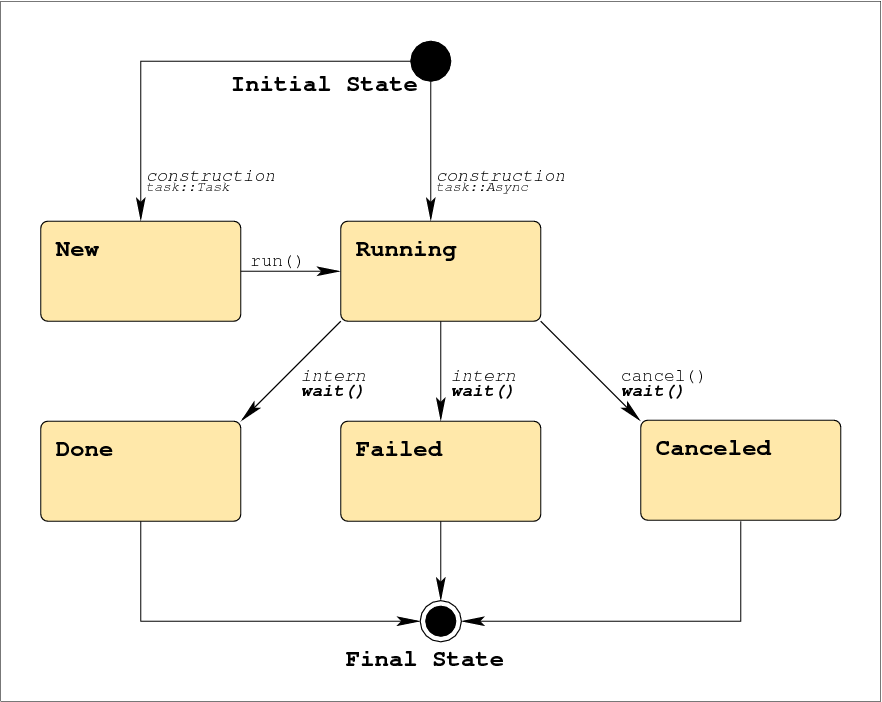
\includegraphics[height=\textheight]{Pics/task_states.eps}
   \end{center}
 \end{slide}

 %%%%%%%%%%%%%%%%%%%%%%%%%%%%%%%%%%%%%%%%%%%%%%%%%%%%%%%%%%%

 \begin{slide}{SAGA: Job States}
   \begin{center}
   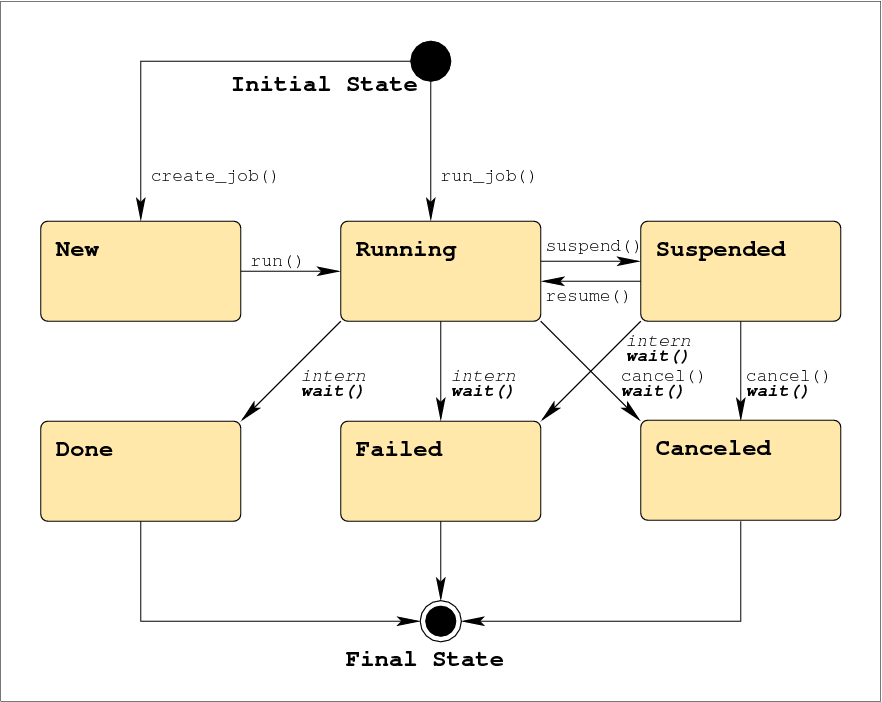
\includegraphics[height=\textheight]{Pics/job_states.eps}
   \end{center}
 \end{slide}

 %%%%%%%%%%%%%%%%%%%%%%%%%%%%%%%%%%%%%%%%%%%%%%%%%%%%%%%%%%%

 \begin{slide}{SAGA: Task States}
   \begin{center}
   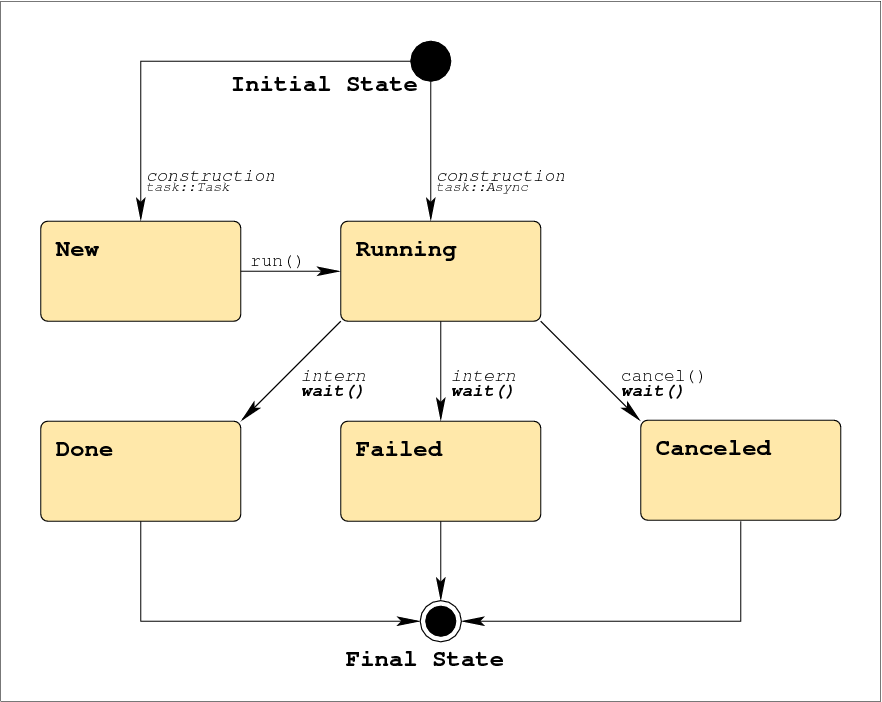
\includegraphics[height=\textheight]{Pics/task_states.eps}
   \end{center}
 \end{slide}

 %%%%%%%%%%%%%%%%%%%%%%%%%%%%%%%%%%%%%%%%%%%%%%%%%%%%%%%%%%%

 \begin{slide}{SAGA: Tasks}

 \dn 

  \begin{itemize}
   \item different versions for each method call: sync, async, task
   \item signature basically the same
   \item differ in state of task returned by that method
  \end{itemize}

 \end{slide}

 %%%%%%%%%%%%%%%%%%%%%%%%%%%%%%%%%%%%%%%%%%%%%%%%%%%%%%%%%%%

 \begin{slide}{SAGA Examples: Tasks}

  \begin{mycode}[label=tasks (i)]

  saga::file file ("gsiftp://remote.host.net/data/data.bin");

  // normal, synchronous
  file.copy ("data.bak");  // void

  // async versions, never throw (use 'rethrow' on failure)
  saga::task t1 = file.copy <saga::task::Sync>  ("data.bak.1");
  saga::task t2 = file.copy <saga::task::Async> ("data.bak.2");
  saga::task t3 = file.copy <saga::task::Task>  ("data.bak.3");

  // t1: Done
  // t2: Running
  // t3: New

  \end{mycode}
   
 \end{slide}

 %%%%%%%%%%%%%%%%%%%%%%%%%%%%%%%%%%%%%%%%%%%%%%%%%%%%%%%%%%%

 \begin{slide}{SAGA Examples: Tasks}

  \begin{mycode}[label=tasks (ii)]

  saga::file file ("gsiftp://remote.host.net/data/data.bin");

  // normal, synchronous
  size_t s = file.get_size ();

  // async versions
  saga::task t1 = file.get_size <saga::task::Sync>  ();
  saga::task t2 = file.get_size <saga::task::Async> ();
  saga::task t3 = file.get_size <saga::task::Task>  ();

  // get_result implies wait, and can throw!
  size_t s1 = t1.get_result <size_t> ();
  size_t s2 = t2.get_result <size_t> ();
  size_t s3 = t3.get_result <size_t> ();

  \end{mycode}
   
 \end{slide}

 %%%%%%%%%%%%%%%%%%%%%%%%%%%%%%%%%%%%%%%%%%%%%%%%%%%%%%%%%%%

 \begin{slide}{SAGA Examples: Tasks}

  \begin{mycode}[label=tasks (iii)]
  
  t3.run ();

  cout << t3.get_state () << endl;  // Running

  t2.wait ();
  t3.wait ();

  // t1, t2, t3: Done (or Failed...)

  \end{mycode}
   
 \end{slide}

 %%%%%%%%%%%%%%%%%%%%%%%%%%%%%%%%%%%%%%%%%%%%%%%%%%%%%%%%%%%

 \begin{slide}{SAGA Examples: Tasks}

  \begin{mycode}[label=tasks container]
  
  saga::task_container tc;

  tc.add (t1);
  tc.add (t2);
  tc.add (t3);

  tc.run  ();
  
  saga::task done_task = tc.wait (Any);

  tc.wait (All);

  \end{mycode}
   
 \end{slide}

 %%%%%%%%%%%%%%%%%%%%%%%%%%%%%%%%%%%%%%%%%%%%%%%%%%%%%%%%%%%

 \begin{slide}{SAGA Examples: Tasks}

  \begin{mycode}[label=tasks and jobs]

  saga::task task = file.copy <saga::task::Asyn> ("b");
  saga::job  job  = js.run_job ("remote.host.net", "/bin/date");
  
  task.add_callback ("State", my_cb);
  job.add_callback  ("State", my_cb);

  saga::task_container tc;

  tc.add (task);
  tc.add (job);

  tc.wait ();

  \end{mycode}
   
 \end{slide}

 
 %%%%%%%%%%%%%%%%%%%%%%%%%%%%%%%%%%%%%%%%%%%%%%%%%%%%%%%%%%%
 
 \begin{slide}{SAGA}
 
  \dn\dn\dn\dn\dn
 
  \begin{center}
   \Large - - - 
  \end{center}
 
 \end{slide}
 
 %%%%%%%%%%%%%%%%%%%%%%%%%%%%%%%%%%%%%%%%%%%%%%%%%%%%%%%%%%%

 \begin{slide}{SAGA planned extensions}
 \dn
  \begin{itemize}
   \item service discovery\\
   \item message based communication\\
   \item information service (Advert Service)\\
   \item resource discovery and management\\
   \item checkpoint \& recovery (GridCPR)\\
  \end{itemize}
 \end{slide}

 %%%%%%%%%%%%%%%%%%%%%%%%%%%%%%%%%%%%%%%%%%%%%%%%%%%%%%%%%%%

 \begin{slide}{SAGA v2: Messages}

  \begin{mycode}[label=Messaging\, server]
  saga::sender snd ("tcp://localhost:1234");

  saga::msg msg;

  msg.set_size (100); // arbitrary size!
  msg.set_data ("abcd...");

  sc.send (msg);
  \end{mycode}

  \dn

  \begin{mycode}[label=Messaging\, client]
  char buf [13];
  saga::receiver rec ("tcp://remote.host.net:1234");

  // int size = rec.test ();
  
  saga::msg = rec.receive (); // internal buffer allocation
  \end{mycode}
   
 \end{slide}

 %%%%%%%%%%%%%%%%%%%%%%%%%%%%%%%%%%%%%%%%%%%%%%%%%%%%%%%%%%%

 \begin{slide}{SAGA v2: Messages}
 \dn
  \begin{itemize}
   \item messages are received intact or not at all
   \item implies protocol, but is silent about interop
   \item async zero copy implementation is possible
  \end{itemize}
 \end{slide}

 %%%%%%%%%%%%%%%%%%%%%%%%%%%%%%%%%%%%%%%%%%%%%%%%%%%%%%%%%%%

 \begin{slide}{SAGA v2: CPR}
 \dn
  \begin{itemize}
   \item no examples yet, API in flux (serice spec in flux)
   \item allows to manage (find, move, stage, archive) checkpoints
   \item allows to trigger checkpointing of jobs
   \item probably name space based, with notification on CP creation
  \end{itemize}
 \end{slide}

 %%%%%%%%%%%%%%%%%%%%%%%%%%%%%%%%%%%%%%%%%%%%%%%%%%%%%%%%%%%

 \begin{slide}{}
 
 \dn\dn\dn\dn\dn
 \begin{center}
  \Huge \B{Questions about API?}\\[10mm]
  \Huge \B{Comments?}\\[10mm]
 \end{center}
 
 \end{slide}
 
 %%%%%%%%%%%%%%%%%%%%%%%%%%%%%%%%%%%%%%%%%%%%%%%%%%%%%%%%%%%

 \begin{slide}{Implementation}
   \includegraphics[width=\textwidth]{Pics/saga_architecture.eps}
 \end{slide}

 %%%%%%%%%%%%%%%%%%%%%%%%%%%%%%%%%%%%%%%%%%%%%%%%%%%%%%%%%%%

 \begin{slide}{Implementation Status}

  \up

  \begin{itemize}

   \item C++
    \begin{itemize}
     \item complete implementation by CCT/VU
     \item in sync with spec, work in progress
     \item other language bindings planned on top\\
           (C, Python, Perl, .Net)
    \end{itemize}

   \item Java (out of sync with the spec)
    \begin{itemize}
     \item partial implementation (jobs, files) by DEISA/EPCC
     \item complete implementation by OMII-UK
     \item possible complete implementation at VU
    \end{itemize}

   \item MiddleWare Bindings
    \begin{itemize}
     \item DEISA/EPCC binds to DEISA
     \item OMII-UK binds to OMII stack, but is flexible
     \item C++ adaptor based -- GT4 and XtreemOS planned
    \end{itemize}

  \end{itemize}

 \end{slide}

 %%%%%%%%%%%%%%%%%%%%%%%%%%%%%%%%%%%%%%%%%%%%%%%%%%%%%%%%%%%

 \begin{slide}{}
 
 
 \begin{center}
  \large \B{Contact}\\[10mm]
 \end{center}

 \T{http://forge.ggf.org/sf/projects/saga-core-wg}\\[10mm]

 $\longrightarrow$ wiki, CVS details

 
 \end{slide}
 
 %%%%%%%%%%%%%%%%%%%%%%%%%%%%%%%%%%%%%%%%%%%%%%%%%%%%%%%%%%%

 \begin{slide}{}
 
 \dn\dn\dn\dn\dn\dn\dn
 \begin{center}
  \Huge \B{Questions?}\\[10mm]
 \end{center}
 
 \end{slide}
 
 %%%%%%%%%%%%%%%%%%%%%%%%%%%%%%%%%%%%%%%%%%%%%%%%%%%%%%%%%%%

 \begin{slide}{}
 
 \dn\dn\dn\dn\dn\dn\dn
 \begin{center}
  \Huge \B{Backup Slides}\\[10mm]
 \end{center}
 
 \end{slide}
 
 %%%%%%%%%%%%%%%%%%%%%%%%%%%%%%%%%%%%%%%%%%%%%%%%%%%%%%%%%%
 
 \begin{slide}{Recap: Grid Applications}
 
  \dn
  Types of Grid Applications
  \dn
 
  \begin{enumerate}
   \item legacy applications
   \item legacy distributed applications
   \item Grid aware applications
  \end{enumerate}
 
 \end{slide}
 
 %%%%%%%%%%%%%%%%%%%%%%%%%%%%%%%%%%%%%%%%%%%%%%%%%%%%%%%%%%
 
 \begin{slide}{Legacy Applications}
 
  \dn
 
  \begin{itemize}
   \item no access to application code
   \item virtualization of heterogenuity
   \item use cases: remote resource utilization, high throughput
   \item \B{favourite technique:} sandboxing (virtualization)
   \item no need for Grid APIs (application exists, non-mutable)\\[2em]
   \item \I{not a topic for this tutorial}
  \end{itemize}
 
 \end{slide}
 
 %%%%%%%%%%%%%%%%%%%%%%%%%%%%%%%%%%%%%%%%%%%%%%%%%%%%%%%%%%
 
 \begin{slide}{Legacy Distributed Applications}
 
  \dn
 
  \begin{itemize}
   \item aware of distribution (MPI, CORBA, ...)
   \item not aware of Grid properties (VO)
   \item usually not very dynamic or adaptive (bootstrapping!)
   \item use cases: scientific applications, bussiness applications
   \item \B{favourite technique:} emulation (GridMPI, etc.)
   \item no need for \I{new} Grid APIs (APIs non-mutable)\\[2em]
   \item \I{not a topic for this tutorial}
  \end{itemize}
 
 \end{slide}
 
 %%%%%%%%%%%%%%%%%%%%%%%%%%%%%%%%%%%%%%%%%%%%%%%%%%%%%%%%%%
 
 \begin{slide}{Grid Aware Applications}
 
  \dn
 
  \begin{itemize}
   \item aware of distribution, heterogeneity, VOs, elasticity etc.
   \item often dynamic and adaptive structure
   \item use cases: collaborative, adaptivite, auto-optimized, scalabile, ...
   \item \B{favourite technique:} depends on structure, middleware, ...
   \item need for Grid APIs (see Part 1)\\[2em] 
   \item \I{topic for this tutorial ~~ :-)}
  \end{itemize}
 
 \end{slide}
 
 %%%%%%%%%%%%%%%%%%%%%%%%%%%%%%%%%%%%%%%%%%%%%%%%%%%%%%%%%

 \begin{slide}{Grid APIs: Globus (pre-WS)}
  \begin{itemize}
   \item low level API for the Globus Grid Middleware
   \item scope reflects Globus services:
    \begin{itemize}
     \item GridFTP
     \item GRAM
     \item MDS
     \item Replicas
    \end{itemize}
    \item some low level API abstractions (xio, gss-assist)
    \item \B{CoG} provides higher level API abstraction for Globus (Java)
  \end{itemize}

 \end{slide}

 %%%%%%%%%%%%%%%%%%%%%%%%%%%%%%%%%%%%%%%%%%%%%%%%%%%%%%%%%%%

 \begin{slide}{GridFTP Example}

  \begin{mycode}[label=GridFTP: Connection Setup]

  globus_module_activate (GLOBUS_FTP_CLIENT_MODULE);
  
  globus_ftp_client_handleattr_init        (&handle_attr);

  globus_ftp_client_handle_init            (&handle, &handle_attr);
  globus_ftp_client_handle_cache_url_state (&handle, server.c_str());

  \end{mycode}
   
 \end{slide}

 %%%%%%%%%%%%%%%%%%%%%%%%%%%%%%%%%%%%%%%%%%%%%%%%%%%%%%%%%%%

 \begin{slide}{GridFTP Example (ii)}

  \begin{mycode}[label=GridFTP: Get File Size]

  globus_ftp_client_operationattr_init     (&attr);
  globus_ftp_client_operationattr_set_mode (&attr, ...);
  
  globus_off_t    size    = GLOBUS_NULL;
  globus_result_t success = globus_ftp_client_size 
                                  (&handle,
                                   url.c_str(),
                                   &attr,
                                   &size,
                                   GLOBUS_NULL, // done_callback,
                                   GLOBUS_NULL);
  if (success != GLOBUS_SUCCESS)
  { ... }

  \end{mycode}
  
 \end{slide}

 %%%%%%%%%%%%%%%%%%%%%%%%%%%%%%%%%%%%%%%%%%%%%%%%%%%%%%%%%%%

 \begin{slide}{GridFTP}

  \dn 
  \dn 

  \begin{itemize}
   \item API covers full scope of GridFTP protocol
   \item low level control over connection and operations
   \item allows syncronous and asyncronous calls (callbacks)
  \end{itemize}

 \end{slide}

 %%%%%%%%%%%%%%%%%%%%%%%%%%%%%%%%%%%%%%%%%%%%%%%%%%%%%%%%%%%

 \begin{slide}{GRAM Example}

  \begin{mycode}[label=GRAM: Job Submit]

  globus_gram_client_callback_allow   (callback_func,
                                       (void *) &Monitor,
                                       &callback_contact);

  rc = globus_gram_client_job_request (rm_contact,
                                       job_description,
                                       job_state_mask,
                                       callback_contact,
                                       &job_contact);

  \end{mycode}
  
 \end{slide}

 %%%%%%%%%%%%%%%%%%%%%%%%%%%%%%%%%%%%%%%%%%%%%%%%%%%%%%%%%%%

 \begin{slide}{GRAM}

  \dn 

  \begin{itemize}
   \item API provides full scope of GRAM protocol
   \item low level control over operations
   \item syncronous and asyncronous calls
   \item job details encapsulated in job description (RSL)
  \end{itemize}

 \end{slide}

 %%%%%%%%%%%%%%%%%%%%%%%%%%%%%%%%%%%%%%%%%%%%%%%%%%%%%%%%%%%

 \begin{slide}{GRAM Example (RSL)}

  \begin{mycode}[label=GRAM: RSL example]
  + ( &
      ( directory    = "/home/user/demo" )
      ( jobtype      =  mpi )
      ( executable   = "/home/user/demo/mpi-application" )
      ( maxWallTime  = "10" )
      ( count        = "8" )
      ( architecture = "i386" )
    ) 
    ( &
      ( directory    = "/home/user/demo" )
      ( jobtype      =  mpi )
      ( executable   = "/home/user/demo/mpi-application" )
      ( maxWallTime  = "10" )
      ( count        = "16" )
      ( architecture = "i386" )
      ( resourceManagerContact = "fs2.das2.nikhef.nl" )
  )
  \end{mycode}

 \end{slide}

 %%%%%%%%%%%%%%%%%%%%%%%%%%%%%%%%%%%%%%%%%%%%%%%%%%%%%%%%%%%

 \begin{slide}{GRAM - RSL}

  \dn 

  \begin{itemize}
   \item GRAM comes with its own job / resource description language
   \item most middlewares invent their own languages
   \item requirements are interpreted in several places (resource broker,
   queue manager, \dots)
  \end{itemize}

 \end{slide}

 %%%%%%%%%%%%%%%%%%%%%%%%%%%%%%%%%%%%%%%%%%%%%%%%%%%%%%%%%%%

 \begin{slide}{gLite Example}

  \begin{mycode}[label=gLite: Job Submit]

  client.Delegate (delegID,
                   "https://cream-ce-01:8443/.../CREAMDelegation", 
                   "/tmp/x509up_u202");      
  client.Register ("https://cream-ce-01:8443/.../CREAM",
                   "https://cream-ce-01:8443/.../CREAMDelegation",
                   delegID,                 
                   JobDescriptionBuffer,              
                   "/tmp/x509up_u202",    
                   uploadURL_and_jobID,  
                   0, false);           
  client.Start    ("https://cream-ce-01:8443/.../CREAM",
                   uploadURL_and_jobID[1]);

  \end{mycode}

 \end{slide}

 %%%%%%%%%%%%%%%%%%%%%%%%%%%%%%%%%%%%%%%%%%%%%%%%%%%%%%%%%%%

 \begin{slide}{gLite}

  \dn 

  \begin{itemize}
   \item moves security details to API level
   \item in some sense, is a customized globus like environment
   \item shows its Globus foundations
   \item faithful to the web service paradigm (app-level WSDL)\\
         \RA API reflects gLite service interface
   \item JDL vs. RSL
  \end{itemize}

 \end{slide}

 %%%%%%%%%%%%%%%%%%%%%%%%%%%%%%%%%%%%%%%%%%%%%%%%%%%%%%%%%%%

 \begin{slide}{CoG Example}

  \begin{mycode}[label=CoG: Job Submit]

  String gramContact = "pitcairn.mcs.anl.gov:6722:...";
  String rsl         = "&(executable=...)(...)(...)";
  
  GramJob job = null;
  try {
     job = new GramJob (rsl);
     Gram.request (gramContact,job);
  } 
  catch (GramException e) {
     ...
  }
     
  \end{mycode}

 \end{slide}

 %%%%%%%%%%%%%%%%%%%%%%%%%%%%%%%%%%%%%%%%%%%%%%%%%%%%%%%%%%%

 \begin{slide}{CoG}

  \dn 

  \begin{itemize}
   \item covers same scope as Globus API
   \item hides complexity and API evolution
   \item separates functional and non functional API parts\\[10mm]
   \item new versions provide additional functionality (workflow, GUI, \dots)
   and cover non-globus middleware
  \end{itemize}

 \end{slide}

 %%%%%%%%%%%%%%%%%%%%%%%%%%%%%%%%%%%%%%%%%%%%%%%%%%%%%%%%%%%

 \begin{slide}{GAT Example}

  \begin{mycode}[label=GAT: Job Submit]

  ResourceBroker              rb ();
  SoftwareDescription         sd (("location",  "/bin/ls")
                                  ("arguments", "-l"));

  HardwareDescription         hd (("memory.size",  1024.f)
                                  ("disk.size",    10.f)
                                  ("machine.type", "i686"));

  Job job = broker.SubmitJob (JobDescription (sd, hd));

  \end{mycode}

 \end{slide}

 %%%%%%%%%%%%%%%%%%%%%%%%%%%%%%%%%%%%%%%%%%%%%%%%%%%%%%%%%%%

 \begin{slide}{GAT}
 \dn
  \begin{itemize}
   \item tries to abstract Grid Middleware functionality
   \item tries to hide middleware details
   \item implementable on multiple middleware systems\\[2em]
   \item usability limited by scope of its use cases\\ (historical reasons)
  \end{itemize}
 \end{slide}

\end{document}

